\documentclass[12pt]{beamer}\usepackage[]{graphicx}\usepackage[]{color}
%% maxwidth is the original width if it is less than linewidth
%% otherwise use linewidth (to make sure the graphics do not exceed the margin)
\makeatletter
\def\maxwidth{ %
  \ifdim\Gin@nat@width>\linewidth
    \linewidth
  \else
    \Gin@nat@width
  \fi
}
\makeatother

\definecolor{fgcolor}{rgb}{0.345, 0.345, 0.345}
\newcommand{\hlnum}[1]{\textcolor[rgb]{0.686,0.059,0.569}{#1}}%
\newcommand{\hlstr}[1]{\textcolor[rgb]{0.192,0.494,0.8}{#1}}%
\newcommand{\hlcom}[1]{\textcolor[rgb]{0.678,0.584,0.686}{\textit{#1}}}%
\newcommand{\hlopt}[1]{\textcolor[rgb]{0,0,0}{#1}}%
\newcommand{\hlstd}[1]{\textcolor[rgb]{0.345,0.345,0.345}{#1}}%
\newcommand{\hlkwa}[1]{\textcolor[rgb]{0.161,0.373,0.58}{\textbf{#1}}}%
\newcommand{\hlkwb}[1]{\textcolor[rgb]{0.69,0.353,0.396}{#1}}%
\newcommand{\hlkwc}[1]{\textcolor[rgb]{0.333,0.667,0.333}{#1}}%
\newcommand{\hlkwd}[1]{\textcolor[rgb]{0.737,0.353,0.396}{\textbf{#1}}}%
\let\hlipl\hlkwb

\usepackage{framed}
\makeatletter
\newenvironment{kframe}{%
 \def\at@end@of@kframe{}%
 \ifinner\ifhmode%
  \def\at@end@of@kframe{\end{minipage}}%
  \begin{minipage}{\columnwidth}%
 \fi\fi%
 \def\FrameCommand##1{\hskip\@totalleftmargin \hskip-\fboxsep
 \colorbox{shadecolor}{##1}\hskip-\fboxsep
     % There is no \\@totalrightmargin, so:
     \hskip-\linewidth \hskip-\@totalleftmargin \hskip\columnwidth}%
 \MakeFramed {\advance\hsize-\width
   \@totalleftmargin\z@ \linewidth\hsize
   \@setminipage}}%
 {\par\unskip\endMakeFramed%
 \at@end@of@kframe}
\makeatother

\definecolor{shadecolor}{rgb}{.97, .97, .97}
\definecolor{messagecolor}{rgb}{0, 0, 0}
\definecolor{warningcolor}{rgb}{1, 0, 1}
\definecolor{errorcolor}{rgb}{1, 0, 0}
\newenvironment{knitrout}{}{} % an empty environment to be redefined in TeX

\usepackage{alltt}
%\usepackage{minpage}
\usetheme{Boadilla}
\IfFileExists{upquote.sty}{\usepackage{upquote}}{}
\begin{document}

\title{\textsc{introduction to r} }
\subtitle{Lubor Homolka}
\date{September $6^{\text{th}}$, 2018}
\begin{frame}
\titlepage
\end{frame}

%-----------

\begin{frame}
\frametitle{Data Science Flow}
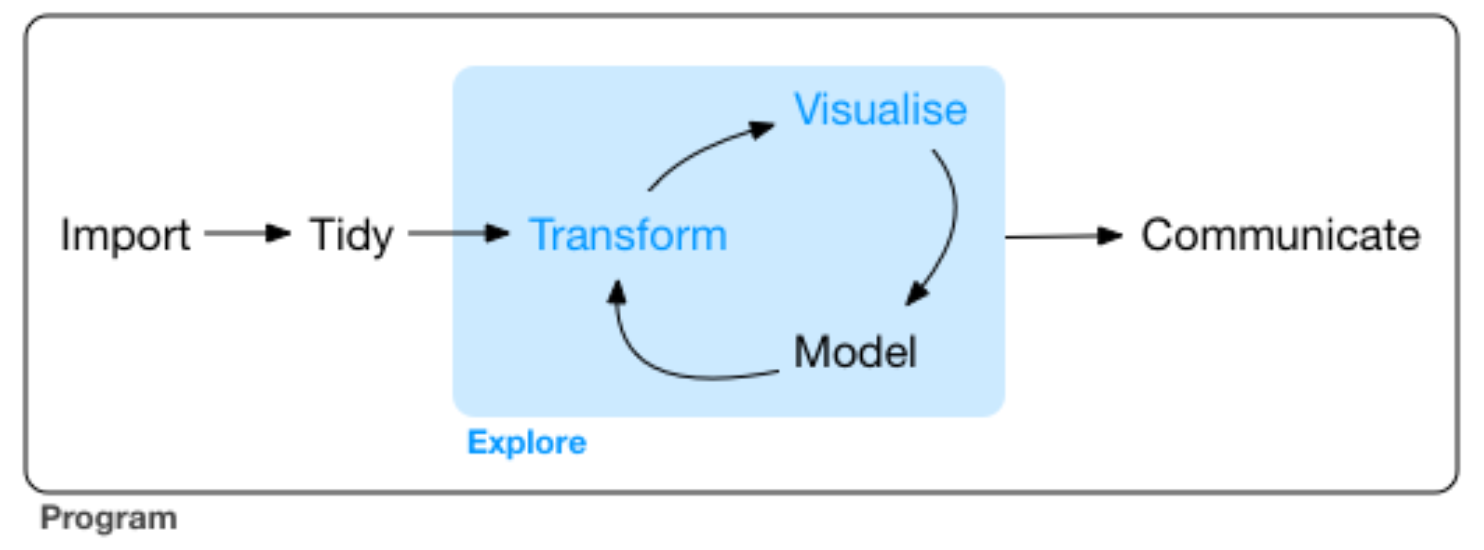
\includegraphics[width=\textwidth,height=\textheight,keepaspectratio]{./Images/01_dataScience}

\flushright{\small
Wickham H, Grolemund G (2010). \textit{R for Data Science}. O'Reilly.
}
\end{frame}

%-----------

\begin{frame}\large
It is often said that 80\% of data analysis is spent on the process of cleaning and preparing
the data (Dasu and Johnson 2003).

\flushright{\small
Dasu T, Johnson T (2003). \textit{Exploratory Data Mining and Data Cleaning}. John Wiley \& Sons.
}
\end{frame}

%-----------
\begin{frame}\Large
\frametitle{Obligatory intro to R and R language...}

Before we start experimenting, we need to talk about:
\begin{itemize}
 \item what is R
 \item basics of object-oriented programming
\end{itemize}

\end{frame}
%-----------

\begin{frame}
\frametitle{R GUI - here you spend the most time...}
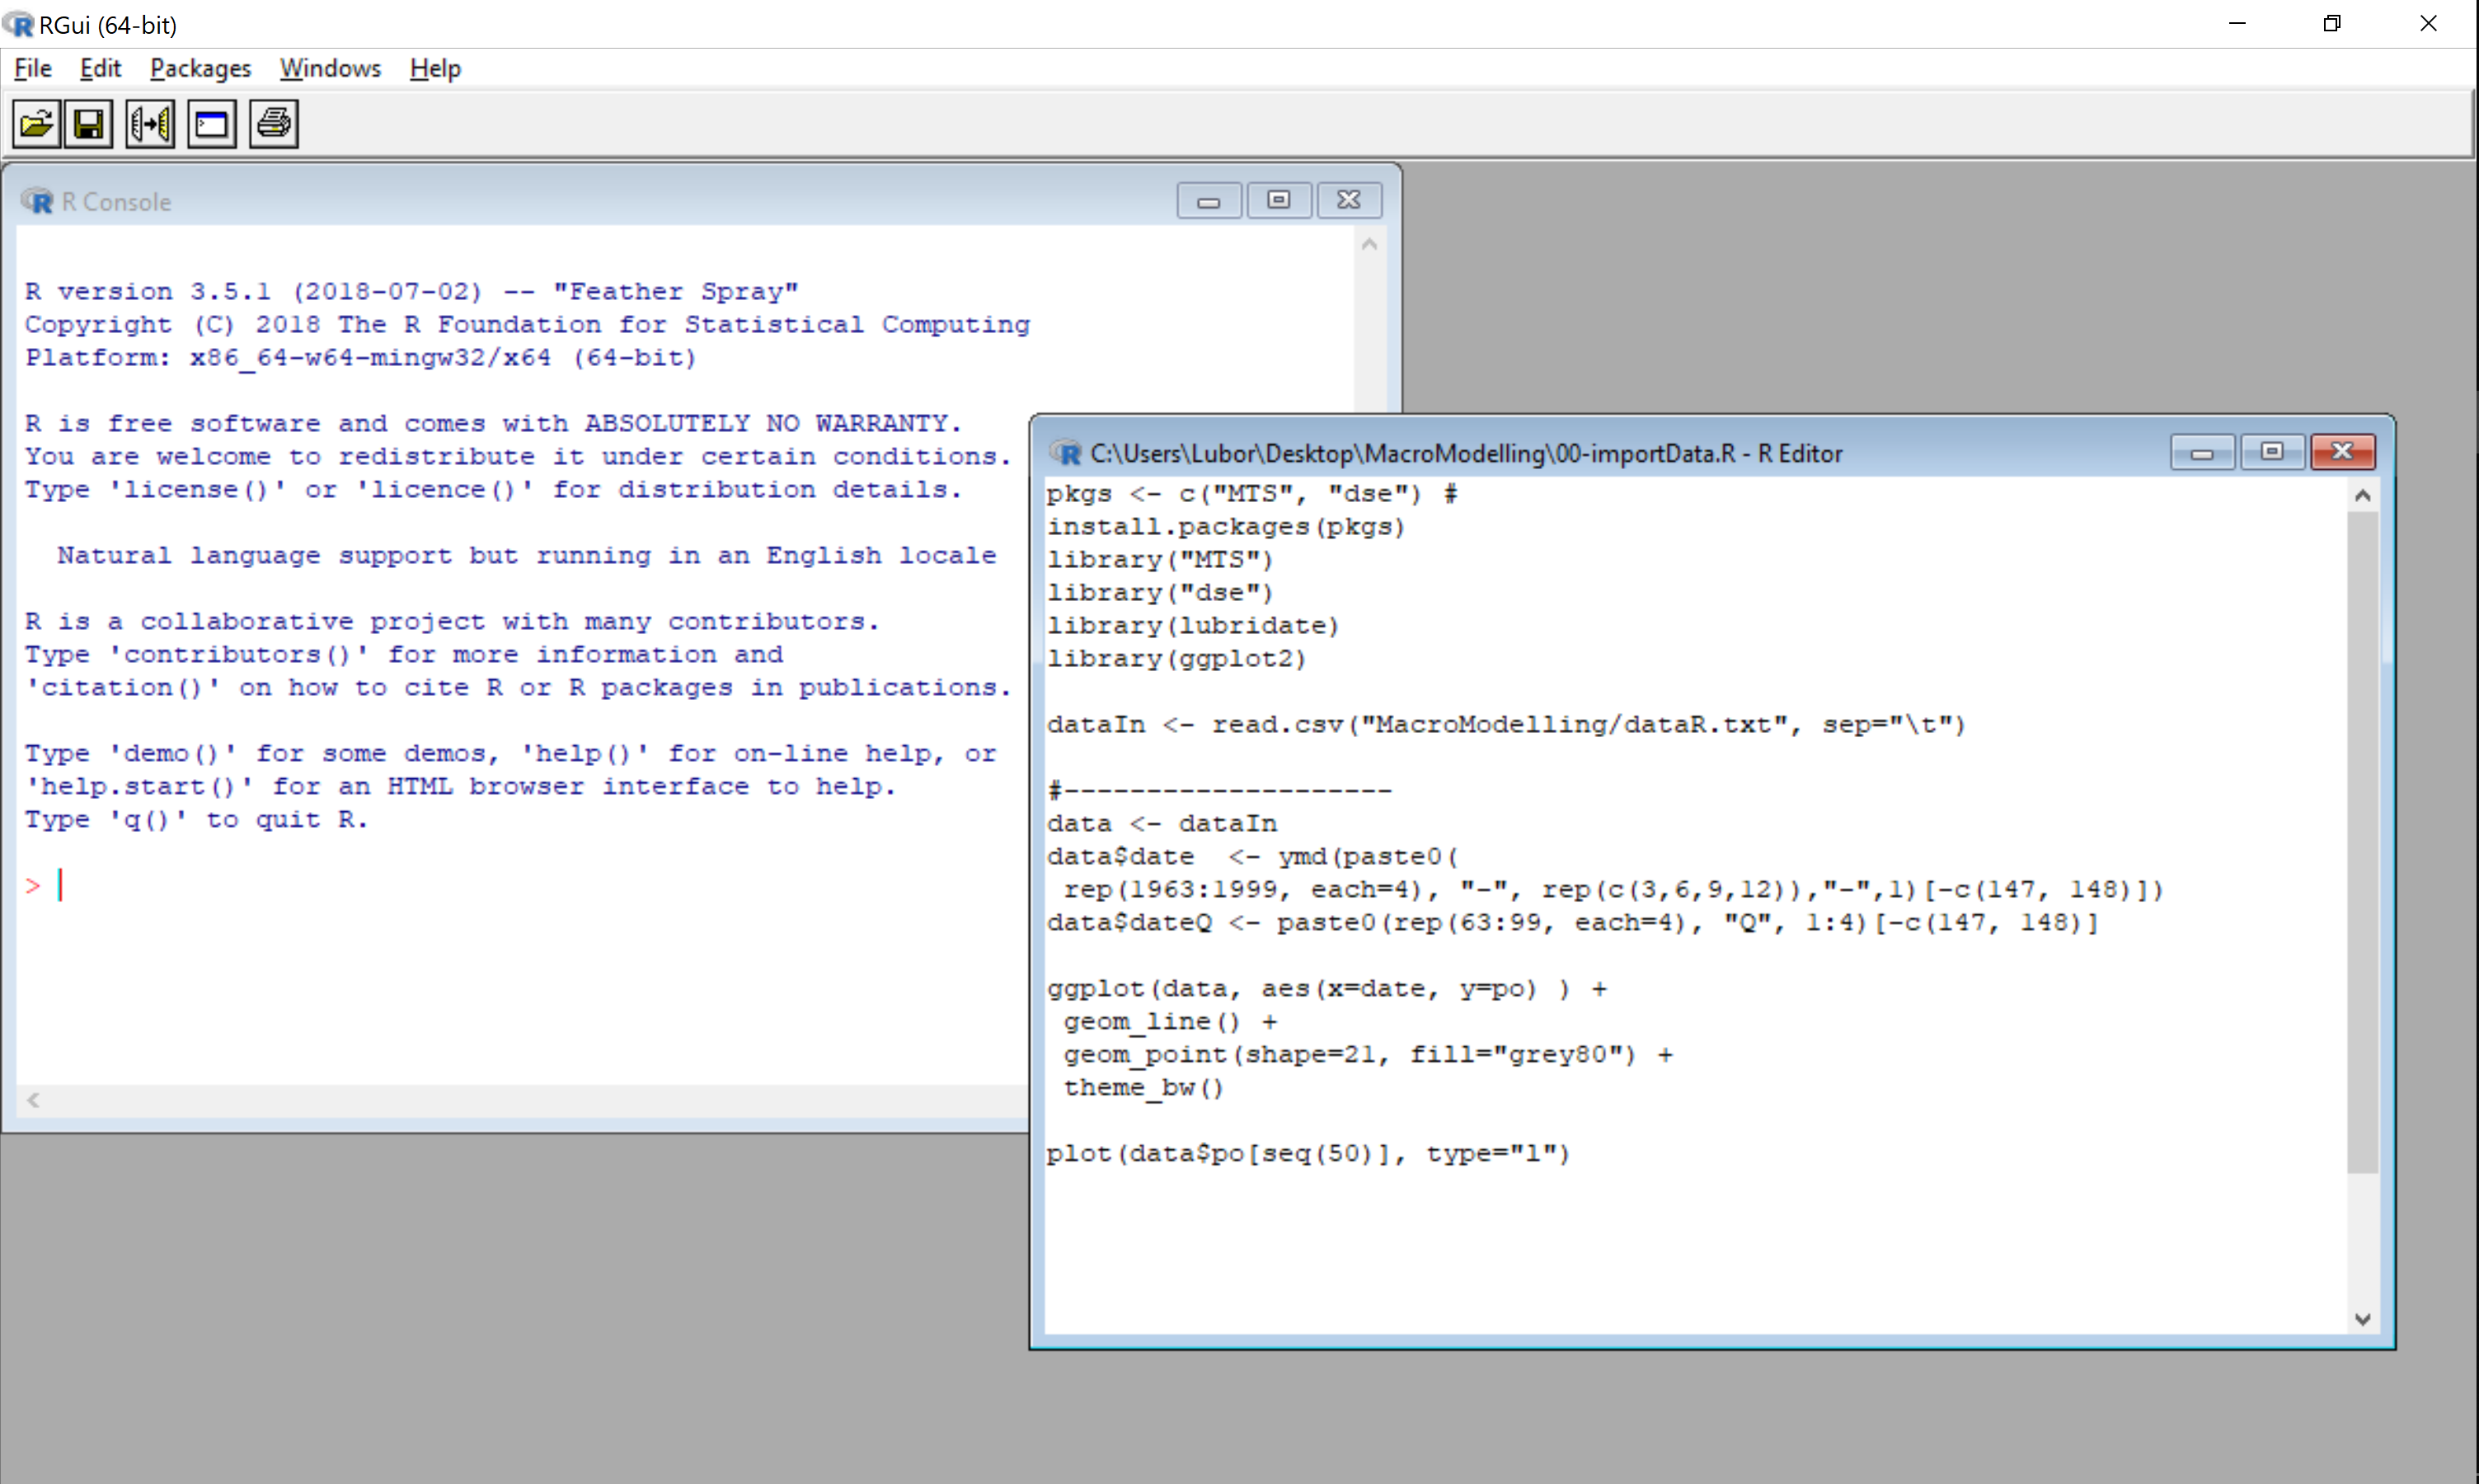
\includegraphics[width=\textwidth,height=\textheight,keepaspectratio]{./Images/02_GUI}
\end{frame}

%-----------

\begin{frame}
\frametitle{... until you need start doing reproducible research}
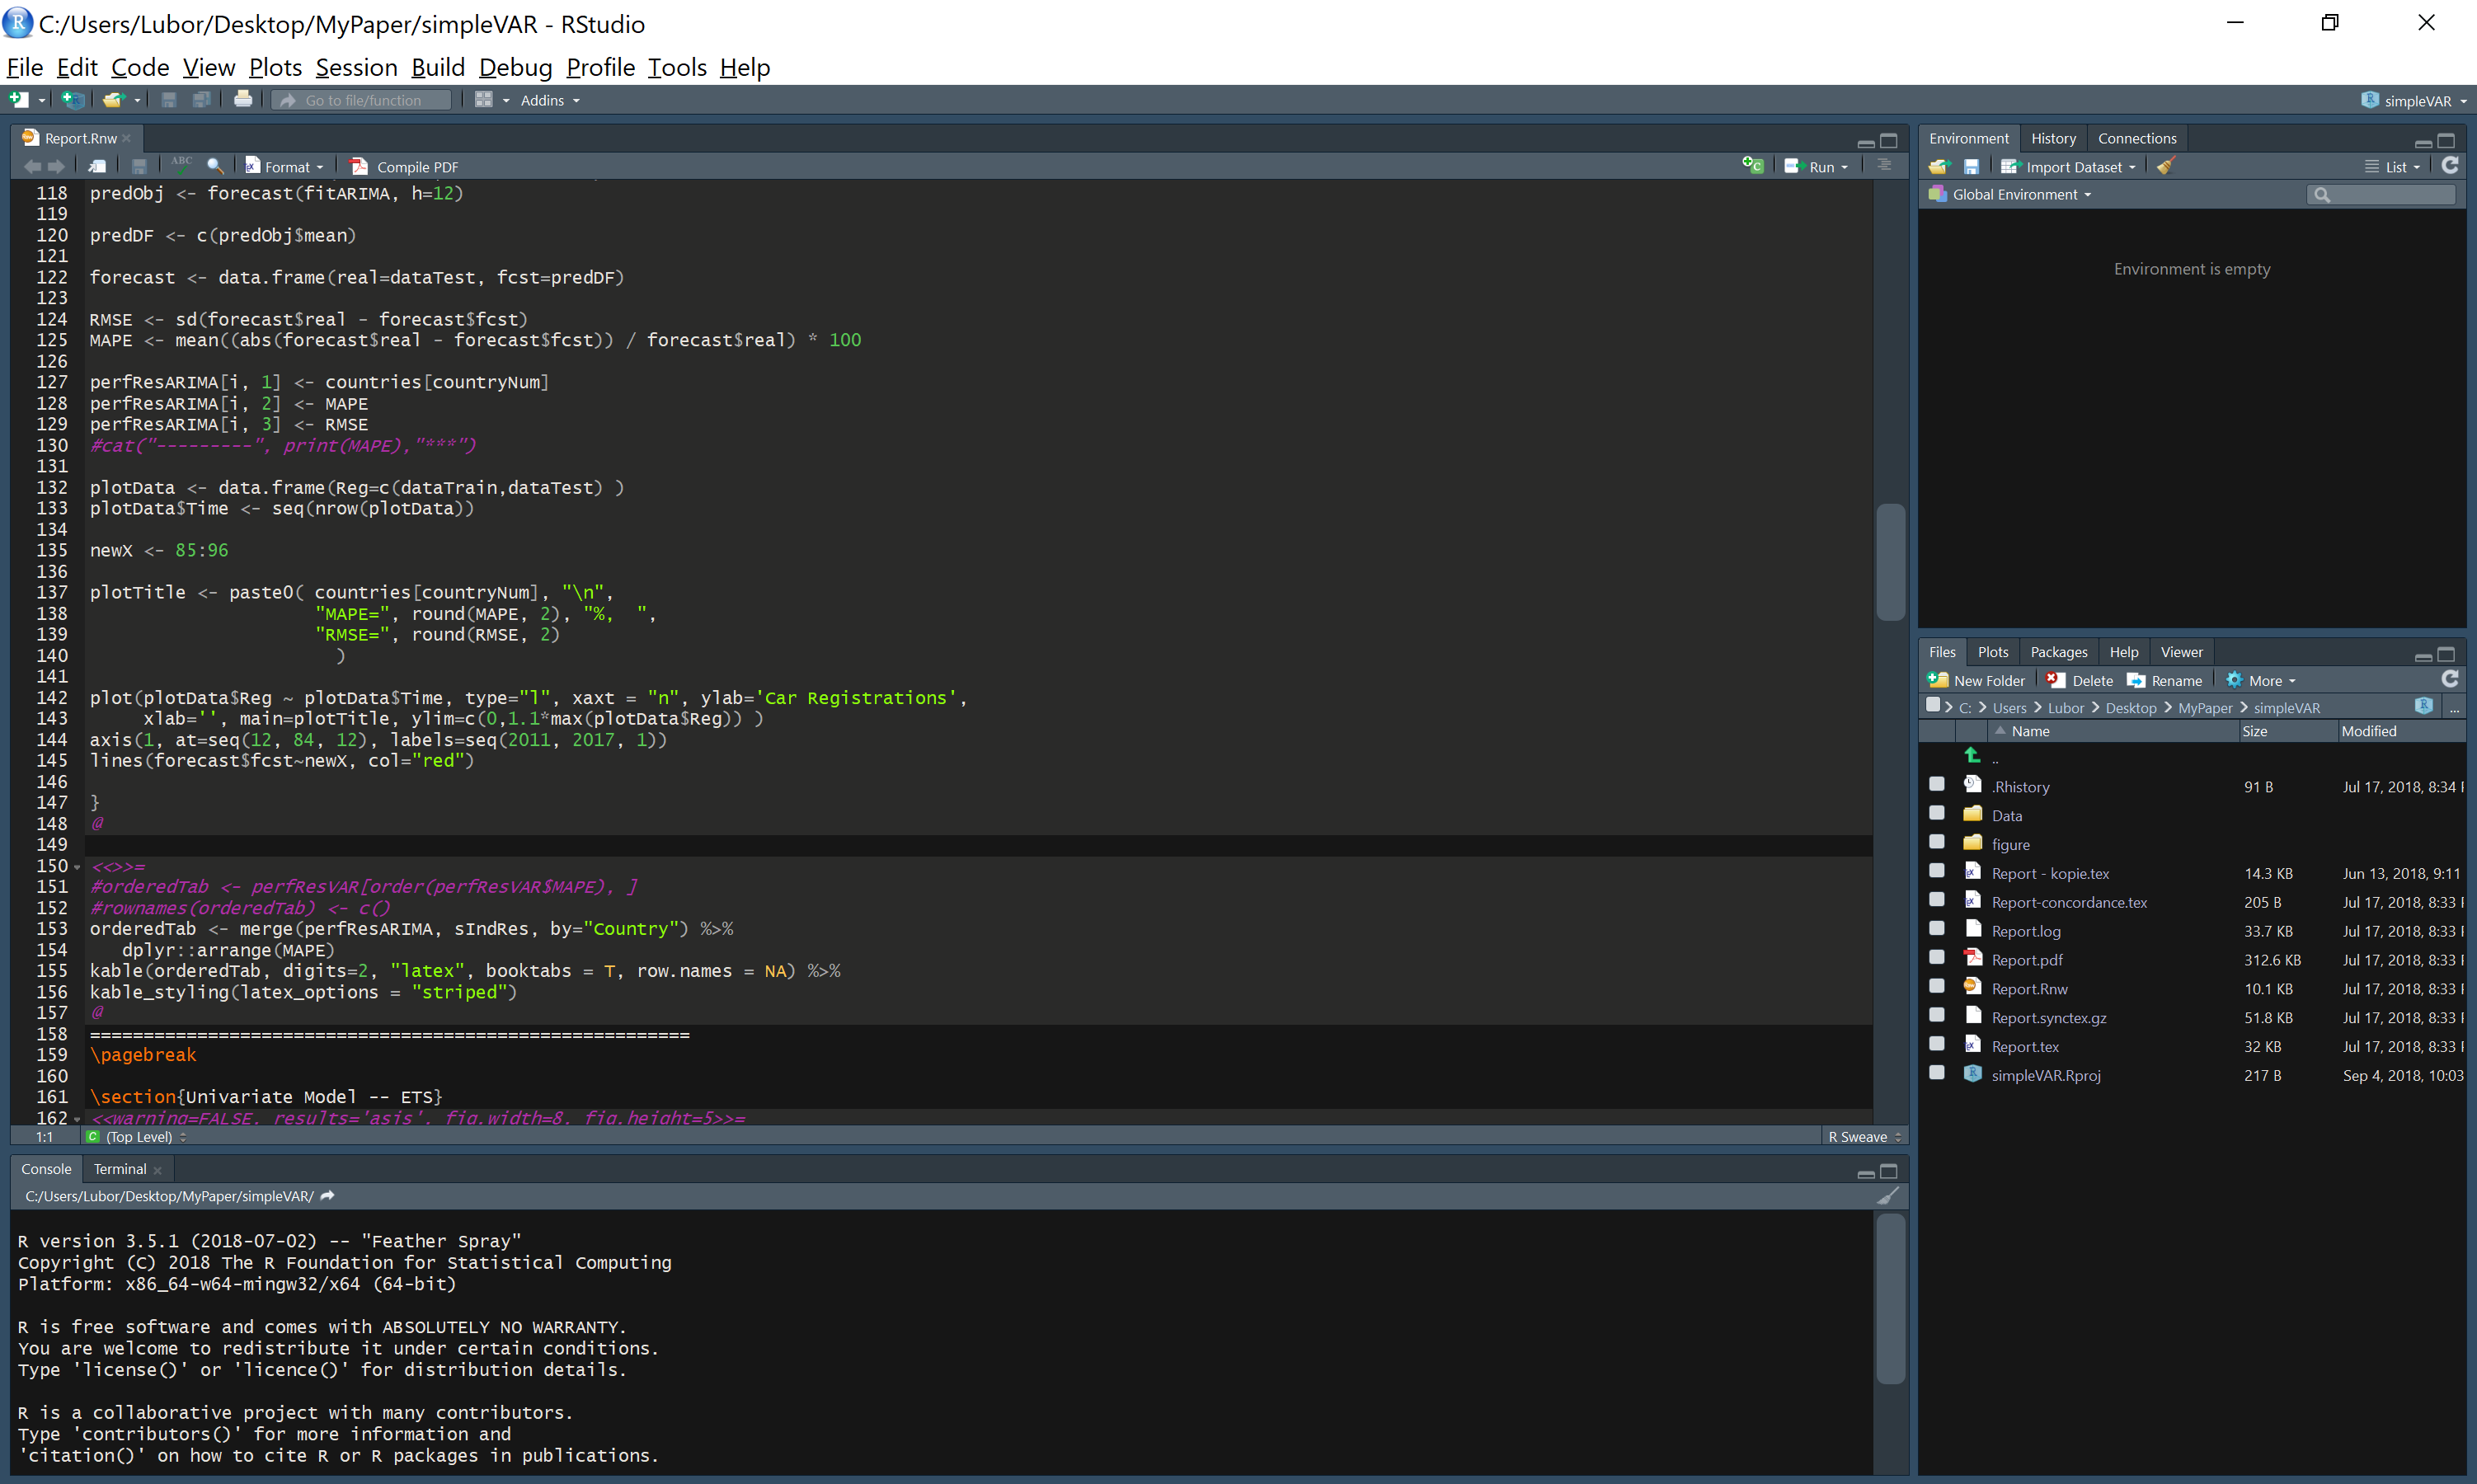
\includegraphics[width=\textwidth,height=\textheight,keepaspectratio]{./Images/03_rStudio}
\end{frame}

%-----------

\begin{frame}[fragile]\large
\frametitle{Object Oriented Programming}

We have 4 students (Alice, Bob, Chelsea and Alice) who form a study group.

\begin{knitrout}
\definecolor{shadecolor}{rgb}{0.969, 0.969, 0.969}\color{fgcolor}\begin{kframe}
\begin{alltt}
\hlstd{names} \hlkwb{<-} \hlkwd{c}\hlstd{(}\hlstr{"Alice"}\hlstd{,} \hlstr{"Bob"}\hlstd{,} \hlstr{"Chelsea"}\hlstd{,} \hlstr{"Alice"}\hlstd{)}
\end{alltt}
\end{kframe}
\end{knitrout}

\textcolor{red}{\texttt{names} is an object.} \onslide<2-> We apply functions on objects:

\begin{knitrout}
\definecolor{shadecolor}{rgb}{0.969, 0.969, 0.969}\color{fgcolor}\begin{kframe}
\begin{alltt}
\hlkwd{unique}\hlstd{(names)}
\end{alltt}
\begin{verbatim}
## [1] "Alice"   "Bob"     "Chelsea"
\end{verbatim}
\end{kframe}
\end{knitrout}

\end{frame}

%-----------

\begin{frame}[fragile]\large
\frametitle{Your turn - open R}

\begin{itemize}
 \item compute $1+1$ \onslide<2->
 \item Click on File $\rightarrow$ New Script. Type $1+1$ into the script and press ctrl+R\onslide<3->
 \item store $1+1$ in object \textcolor{blue}{\texttt{simpleSum}}\onslide<4->
\begin{knitrout}
\definecolor{shadecolor}{rgb}{0.969, 0.969, 0.969}\color{fgcolor}\begin{kframe}
\begin{alltt}
\hlstd{simpleSum} \hlkwb{<-} \hlnum{1}\hlopt{+}\hlnum{1}
\end{alltt}
\end{kframe}
\end{knitrout}
 \item take $\sqrt simpleSum$,  use \textcolor{red}{sqrt()} function\onslide<5->
\begin{knitrout}
\definecolor{shadecolor}{rgb}{0.969, 0.969, 0.969}\color{fgcolor}\begin{kframe}
\begin{alltt}
\hlkwd{sqrt}\hlstd{(simpleSum)}
\end{alltt}
\begin{verbatim}
## [1] 1.414214
\end{verbatim}
\end{kframe}
\end{knitrout}
\end{itemize}

\end{frame}

%-----------

\begin{frame}[fragile]
\frametitle{Data Types}

\begin{itemize}
 \item numeric
 \item character, factor (important for variable coding, allows ordering)
\end{itemize}

\begin{small}
\begin{knitrout}\footnotesize
\definecolor{shadecolor}{rgb}{0.969, 0.969, 0.969}\color{fgcolor}\begin{kframe}
\begin{alltt}
\hlstd{a} \hlkwb{<-} \hlnum{1}
\hlstd{b} \hlkwb{<-} \hlstr{"male"}
\hlstd{c} \hlkwb{<-} \hlstr{"1"}

\hlkwd{class}\hlstd{(a)}
\end{alltt}
\begin{verbatim}
## [1] "numeric"
\end{verbatim}
\begin{alltt}
\hlkwd{class}\hlstd{(b)}
\end{alltt}
\begin{verbatim}
## [1] "character"
\end{verbatim}
\begin{alltt}
\hlkwd{class}\hlstd{(c)}
\end{alltt}
\begin{verbatim}
## [1] "character"
\end{verbatim}
\end{kframe}
\end{knitrout}
\end{small}

\end{frame}

%-----------

\begin{frame}\large
\frametitle{Other Important Types}
What if we want to work with more values at the same time?
\begin{itemize}
 \item column = \texttt{c()}
 \item matrix = \texttt{matrix()}
 \item data frame = \texttt{data.frame()}
 \item list = \texttt{list()}
 \item tibble = \texttt{tibble()}
\end{itemize}
\end{frame}

%-----------

\begin{frame}[fragile]
Do you remember motivating example?

\begin{knitrout}
\definecolor{shadecolor}{rgb}{0.969, 0.969, 0.969}\color{fgcolor}\begin{kframe}
\begin{alltt}
\hlstd{names} \hlkwb{<-} \hlkwd{c}\hlstd{(}\hlstr{"Alice"}\hlstd{,} \hlstr{"Bob"}\hlstd{,} \hlstr{"Chelsea"}\hlstd{,} \hlstr{"Alice"}\hlstd{)}
\end{alltt}
\end{kframe}
\end{knitrout}
\onslide<2->

Try following:
\begin{enumerate}
 \item Create similar column called \textcolor{red}{\texttt{scores}}, which contains number of points from the test on a scale from 0--100 for each student.\onslide<3->
\begin{knitrout}
\definecolor{shadecolor}{rgb}{0.969, 0.969, 0.969}\color{fgcolor}\begin{kframe}
\begin{alltt}
\hlstd{scores} \hlkwb{<-} \hlkwd{c}\hlstd{(}\hlnum{60}\hlstd{,} \hlnum{40}\hlstd{,} \hlnum{55}\hlstd{,} \hlnum{70}\hlstd{)}
\end{alltt}
\end{kframe}
\end{knitrout}
 \item Create \texttt{data.frame(names, scores)} and name it \textcolor{red}{\texttt{classData}}\onslide<4->
\begin{knitrout}
\definecolor{shadecolor}{rgb}{0.969, 0.969, 0.969}\color{fgcolor}\begin{kframe}
\begin{alltt}
\hlstd{classData} \hlkwb{<-} \hlkwd{data.frame}\hlstd{(names, scores)}
\end{alltt}
\end{kframe}
\end{knitrout}
 \item See what is inside of the \texttt{classData} object
 \item Inspect \texttt{classData} by function \textcolor{blue}{\texttt{str()}} \onslide<5->
\begin{knitrout}
\definecolor{shadecolor}{rgb}{0.969, 0.969, 0.969}\color{fgcolor}\begin{kframe}
\begin{alltt}
\hlkwd{str}\hlstd{(classData)}
\end{alltt}
\begin{verbatim}
## 'data.frame':	4 obs. of  2 variables:
##  $ names : Factor w/ 3 levels "Alice","Bob",..: 1 2 3 1
##  $ scores: num  60 40 55 70
\end{verbatim}
\end{kframe}
\end{knitrout}
\end{enumerate}

\end{frame}

%-----------

\begin{frame}[fragile]
\begin{enumerate}
\setcounter{enumi}{4}
 \item Inspect \textcolor{red}{\texttt{classData}} by function \textcolor{blue}{\texttt{summary()}} \onslide<2->
\begin{knitrout}
\definecolor{shadecolor}{rgb}{0.969, 0.969, 0.969}\color{fgcolor}\begin{kframe}
\begin{alltt}
\hlkwd{summary}\hlstd{(classData)}
\end{alltt}
\begin{verbatim}
##      names       scores     
##  Alice  :2   Min.   :40.00  
##  Bob    :1   1st Qu.:51.25  
##  Chelsea:1   Median :57.50  
##              Mean   :56.25  
##              3rd Qu.:62.50  
##              Max.   :70.00
\end{verbatim}
\end{kframe}
\end{knitrout}
\end{enumerate}

\onslide<3-> Summary of the data is an object: 

\begin{knitrout}\footnotesize
\definecolor{shadecolor}{rgb}{0.969, 0.969, 0.969}\color{fgcolor}\begin{kframe}
\begin{alltt}
\hlstd{summaryTab} \hlkwb{<-} \hlkwd{summary}\hlstd{(classData)}
\hlkwd{class}\hlstd{(summaryTab)} \hlcom{# ident. class(summary(classData))}
\end{alltt}
\begin{verbatim}
## [1] "table"
\end{verbatim}
\end{kframe}
\end{knitrout}

\end{frame}

%-----------

\begin{frame}
\frametitle{Try it by yourself}

\begin{enumerate}
 \item generate 200 values from Normal distribution by function \textcolor{blue}{\texttt{rnorm(n=200)}} and store values in \textcolor{red}{\texttt{normData1}}
 \item compute standard deviation \textcolor{blue}{\texttt{sd()}} and mean value \textcolor{blue}{\texttt{mean()}}
 \item create a histogram by \textcolor{blue}{\texttt{hist()}}
 \item generate another 200 values from Normal distribution and store them in object \textcolor{red}{\texttt{normData2}}
 \item create \textcolor{blue}{\texttt{data.frame()}} with 2 columns -- normData1 and normData2 and call it \textcolor{red}{\texttt{normalData}}
 \item create a scatter plot by \textcolor{blue}{\texttt{plot(normalData)}}
 \item compute a correlation of normData1 and normData2, by function \textcolor{blue}{\texttt{cor()}}. If you need help for function, type \texttt{?cor}
\end{enumerate}

\end{frame}

%-----------

\begin{frame}\Huge\centering
Import
\end{frame}

%-----------

\begin{frame}\large
\frametitle{Data Import}

There are several ways how to read data into R:

\begin{itemize}
 \item from your file (text file, Excel file)
 \item from online sources (Eurostat)
 \item other (web scraping through XML)
\end{itemize}

\onslide<2->
\begin{block}{Warning}
  Keeping data in MS Excel makes doing (untracable) changes too tempting!
\end{block}

\end{frame}

%-----------

\begin{frame}[fragile]

\begin{block}{Recommendation}
Create one data file in .txt or .csv filetype. \textcolor{red}{DON'T} change it. Read it into R. Do all manipulations in R. All steps are recorded in the script.
\end{block}

\begin{itemize}
 \item Store the file in \textcolor{blue}{./myRproject/Data} folder \onslide<2->
 \item change R working directory
\end{itemize}
\begin{knitrout}
\definecolor{shadecolor}{rgb}{0.969, 0.969, 0.969}\color{fgcolor}\begin{kframe}
\begin{alltt}
\hlkwd{getwd}\hlstd{()} \hlcom{#to find current WD}
\end{alltt}
\begin{verbatim}
## [1] "C:/Users/Lubor/Disk Google/Work/2018/R_workshop"
\end{verbatim}
\end{kframe}
\end{knitrout}
\onslide<3-> Set the working directory one folder under data folder:
\begin{knitrout}
\definecolor{shadecolor}{rgb}{0.969, 0.969, 0.969}\color{fgcolor}\begin{kframe}
\begin{alltt}
\hlkwd{setwd}\hlstd{(}\hlstr{"C:/Users/Lubor/Rworkshop"}\hlstd{)}
\end{alltt}
\end{kframe}
\end{knitrout}
if your data folder is in "C:/Users/Lubor/Rworkshop/Data"

\end{frame}

%-----------

\begin{frame}
\frametitle{Open carsData.txt}
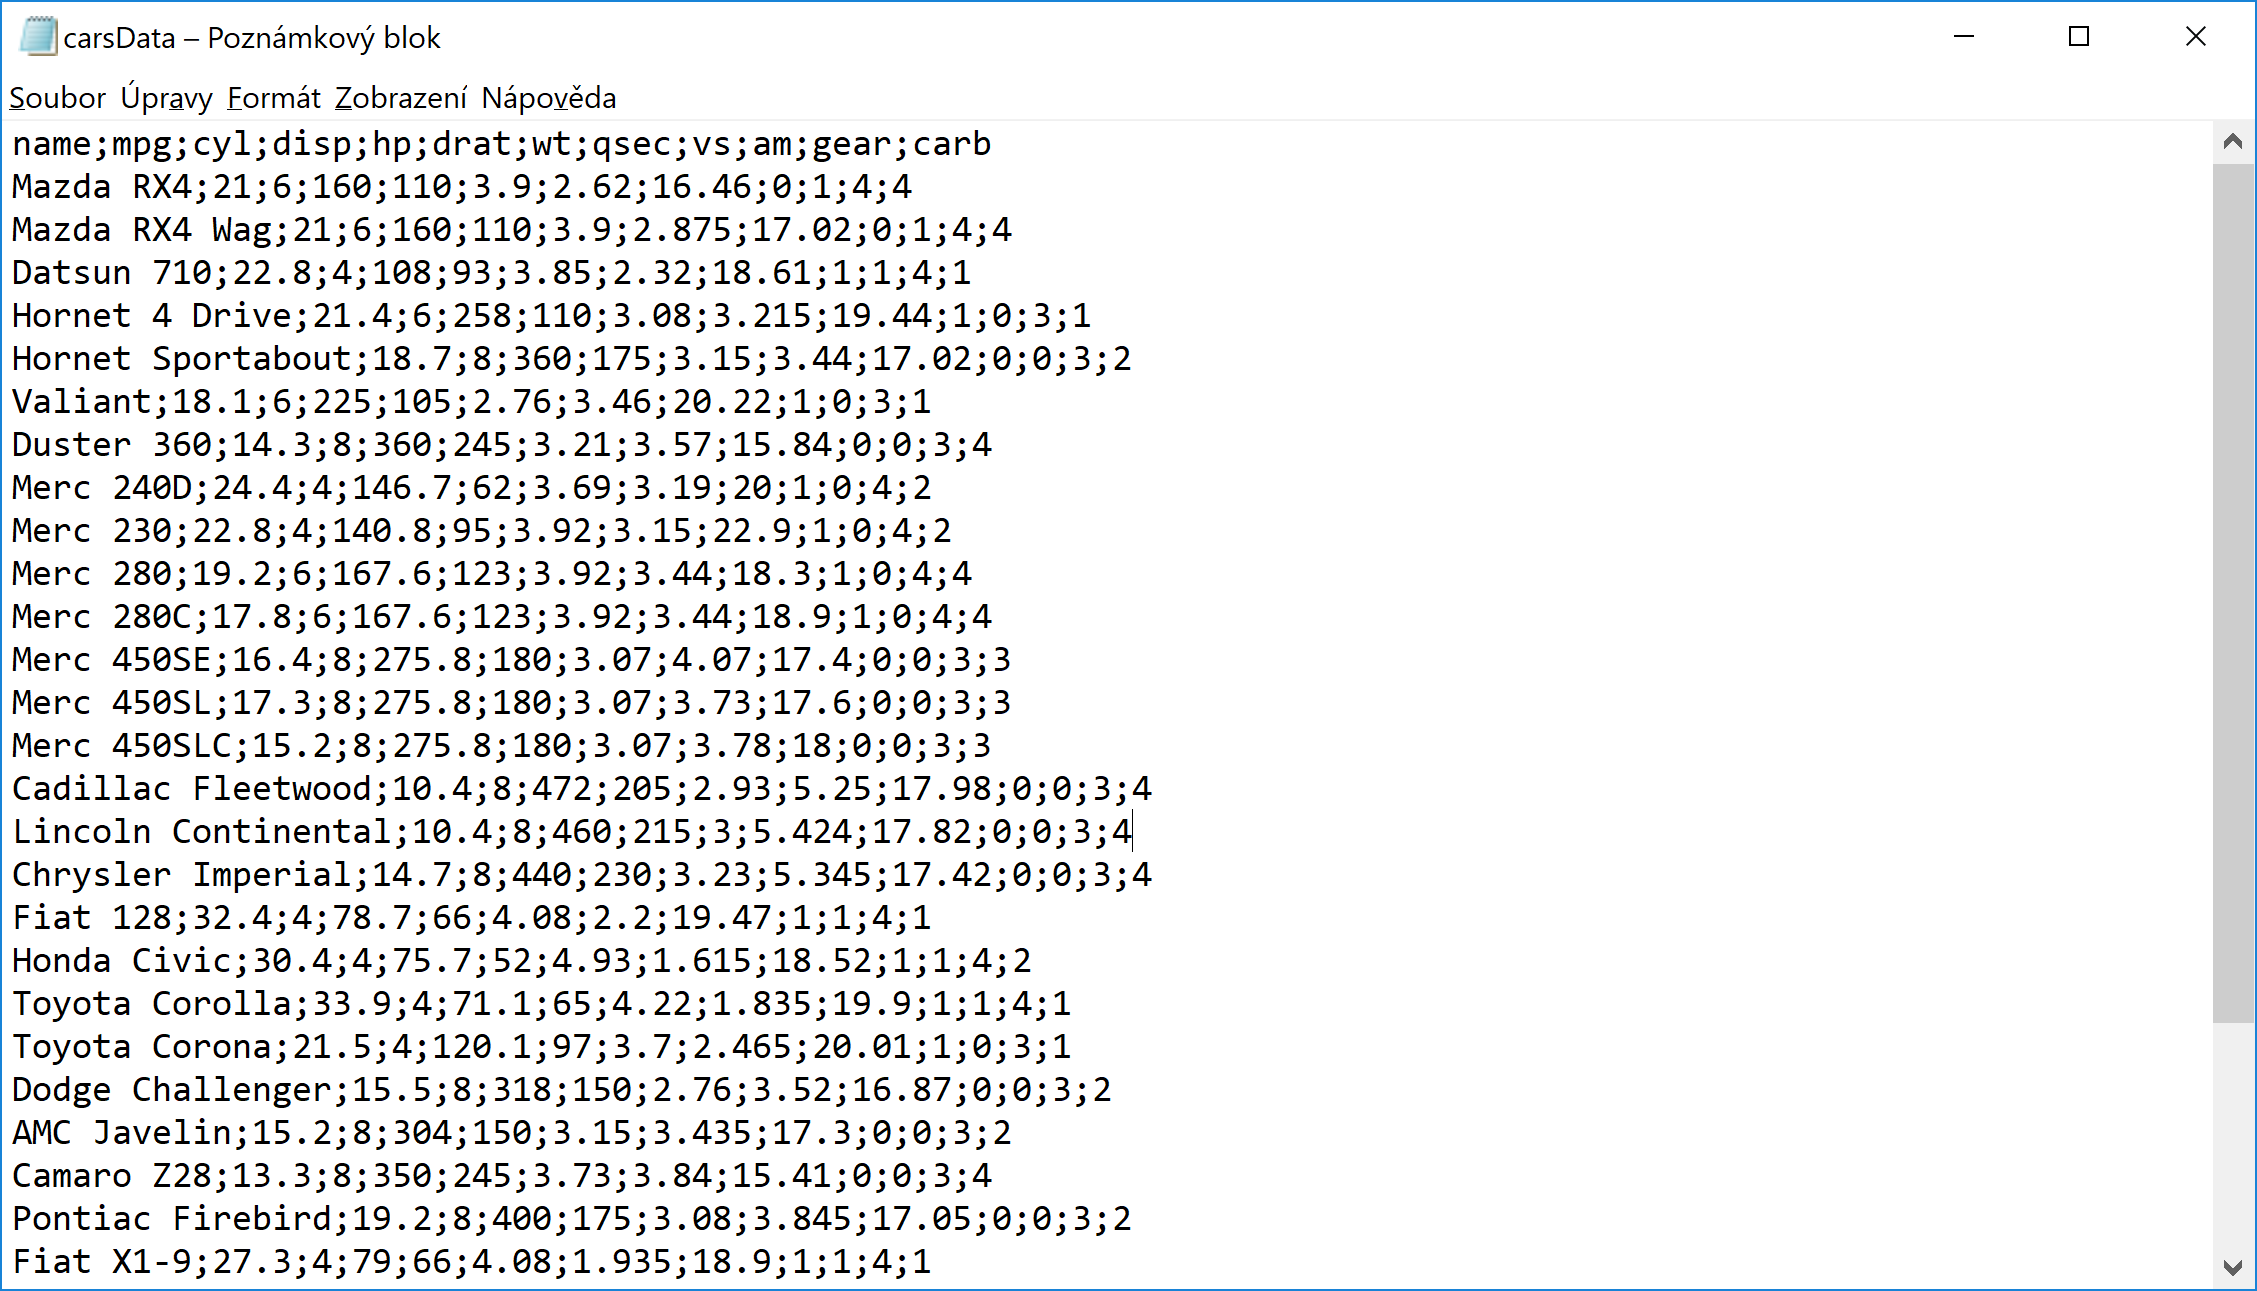
\includegraphics[width=\textwidth,height=\textheight,keepaspectratio]{./Images/04_inspectTXT}

\onslide<2-> How can I create similar file?
\end{frame}

%-----------

\begin{frame}
\frametitle{Use MS Excel}\centering
 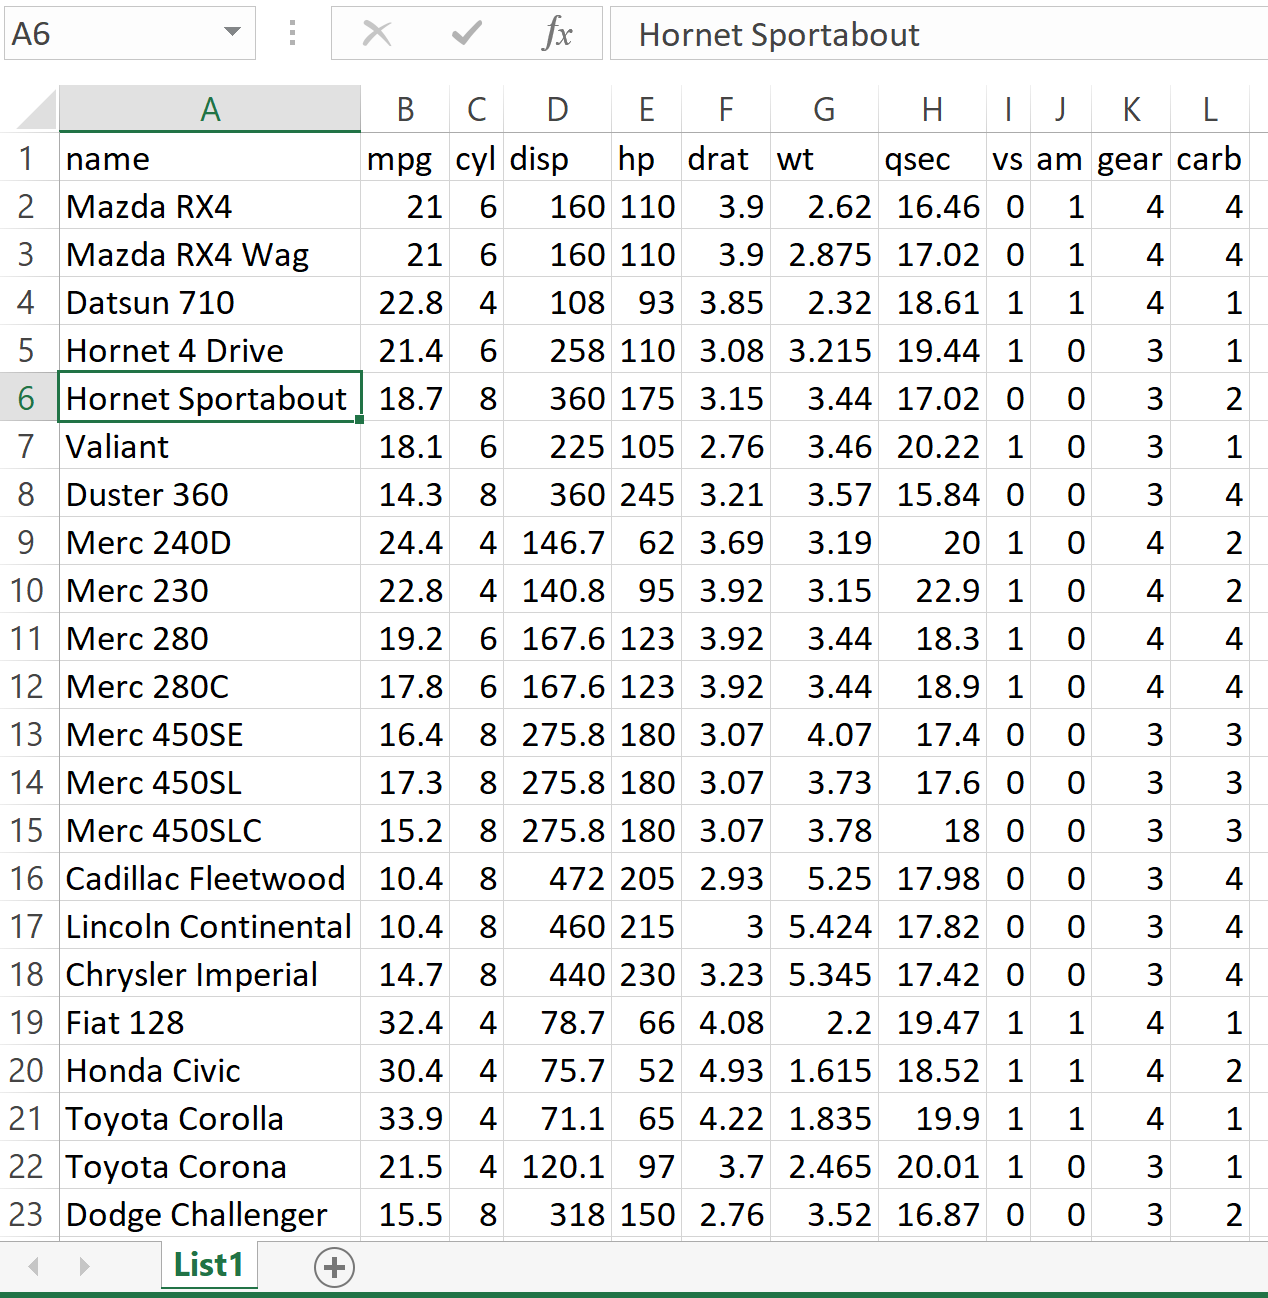
\includegraphics[width=0.8\textwidth,height=0.8\textheight,keepaspectratio]{./Images/05_Excel}
\end{frame}

%-----------

\begin{frame}\centering
\frametitle{Save File as...}
 \includegraphics[width=0.8\textwidth,height=0.8\textheight,keepaspectratio]{./Images/06_saveAS}
\end{frame}

%-----------

\begin{frame}[fragile]
\frametitle{Let's do it!}

\begin{knitrout}
\definecolor{shadecolor}{rgb}{0.969, 0.969, 0.969}\color{fgcolor}\begin{kframe}
\begin{alltt}
\hlkwd{setwd}\hlstd{(}\hlstr{"C:/Users/Lubor/Rworkshop"}\hlstd{)}
\end{alltt}
\end{kframe}
\end{knitrout}

We will use function \textcolor{red}{\texttt{read.table}} and store data in the variable \texttt{dataIn} \onslide<2->

Check the help file of the function:
\begin{knitrout}
\definecolor{shadecolor}{rgb}{0.969, 0.969, 0.969}\color{fgcolor}\begin{kframe}
\begin{alltt}
\hlopt{?}\hlstd{read.table}
\end{alltt}
\end{kframe}
\end{knitrout}
 \centering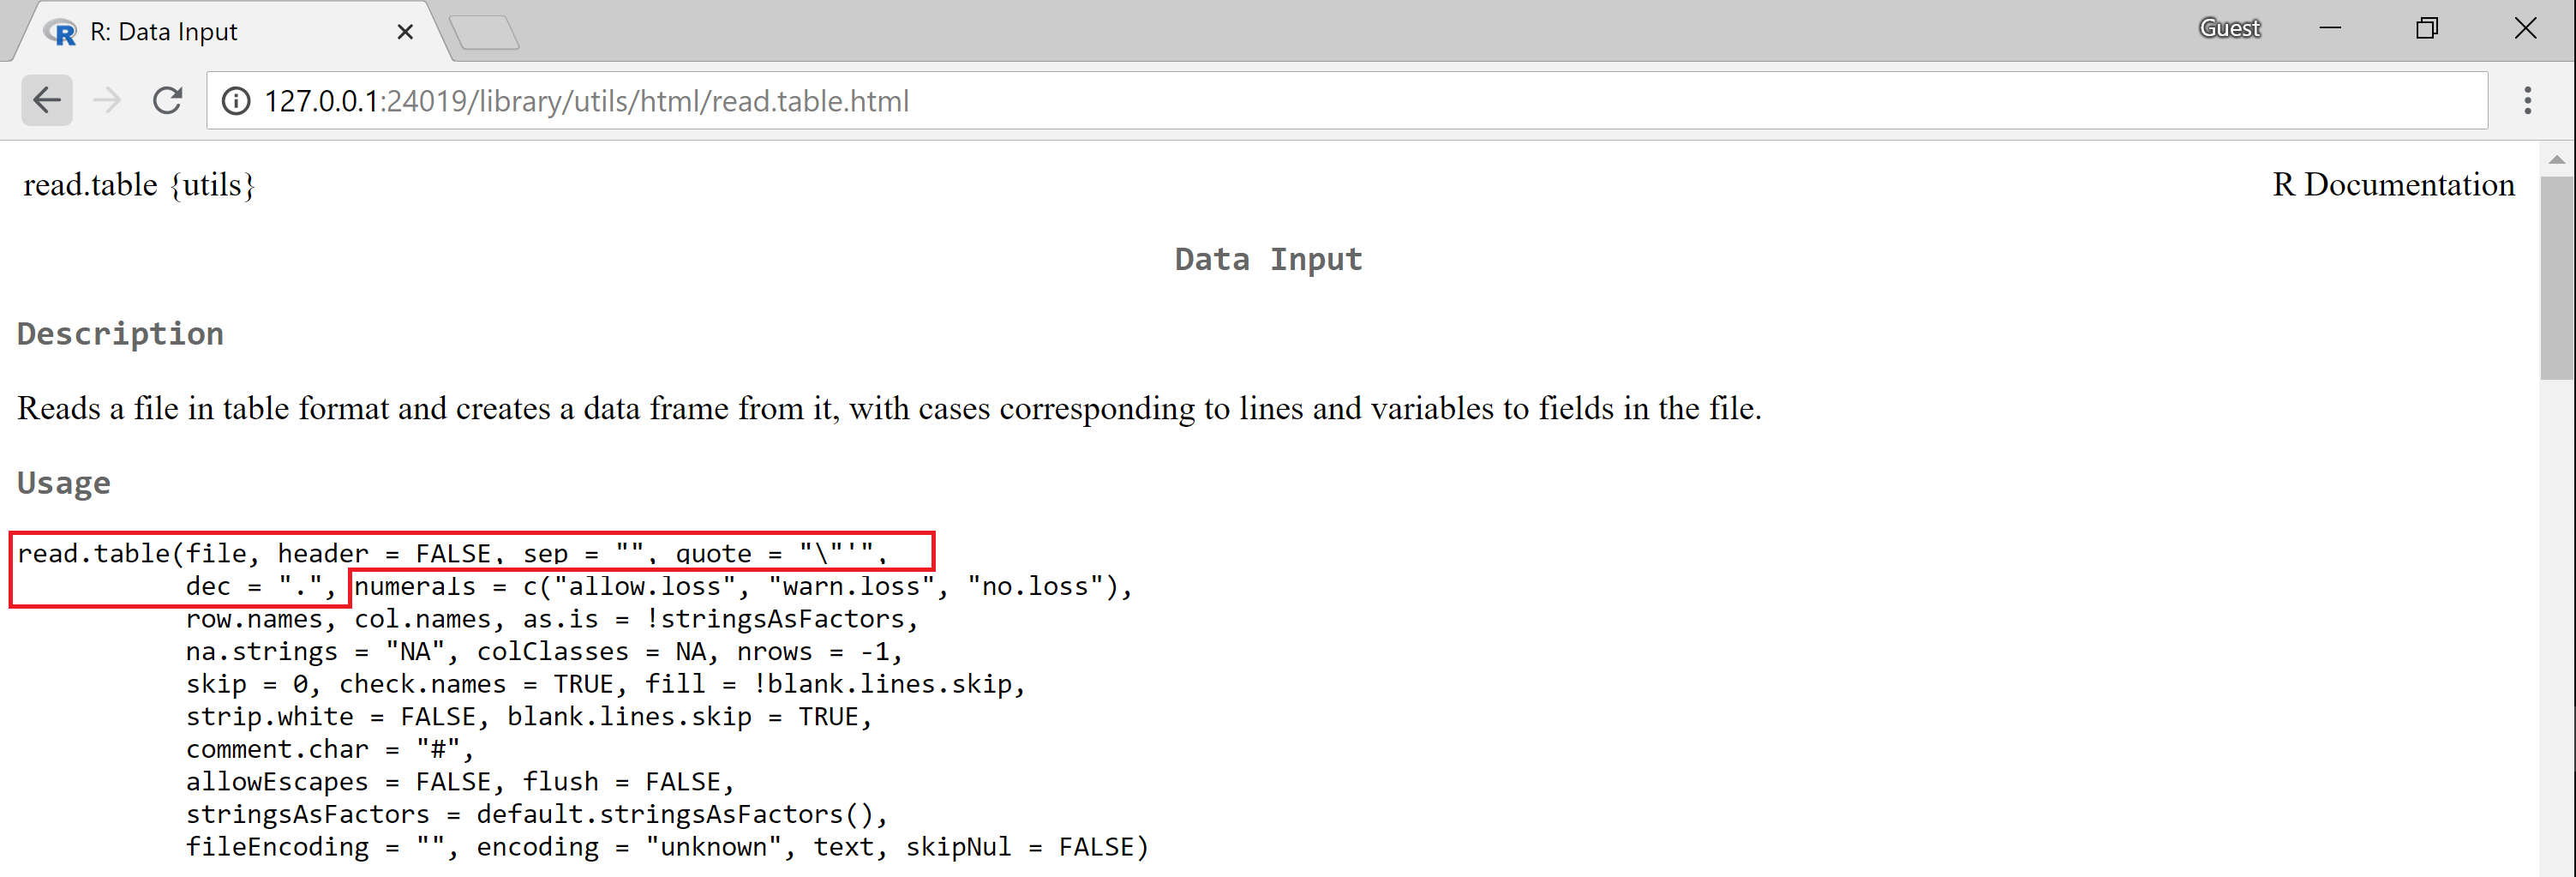
\includegraphics[width=0.8\textwidth,height=0.8\textheight,keepaspectratio]{./Images/07_readTable}

\end{frame}

%-----------

\begin{frame}[fragile]
\frametitle{In our case:}

\begin{knitrout}
\definecolor{shadecolor}{rgb}{0.969, 0.969, 0.969}\color{fgcolor}\begin{kframe}
\begin{alltt}
\hlstd{dataIn} \hlkwb{<-} \hlkwd{read.table}\hlstd{(}\hlstr{"./Data/carsData.txt"}\hlstd{,}
                      \hlkwc{header} \hlstd{=} \hlnum{TRUE}\hlstd{,} \hlkwc{sep}\hlstd{=}\hlstr{";"}\hlstd{)}
\end{alltt}
\end{kframe}
\end{knitrout}
\onslide<2->
Inspect the first 6 rows by function \textcolor{red}{\texttt{head()}} \onslide<2->
\begin{knitrout}
\definecolor{shadecolor}{rgb}{0.969, 0.969, 0.969}\color{fgcolor}\begin{kframe}
\begin{alltt}
\hlkwd{head}\hlstd{(dataIn)}
\end{alltt}
\begin{verbatim}
##                name  mpg cyl disp  hp drat    wt  qsec vs am gear carb
## 1         Mazda RX4 21.0   6  160 110 3.90 2.620 16.46  0  1    4    4
## 2     Mazda RX4 Wag 21.0   6  160 110 3.90 2.875 17.02  0  1    4    4
## 3        Datsun 710 22.8   4  108  93 3.85 2.320 18.61  1  1    4    1
## 4    Hornet 4 Drive 21.4   6  258 110 3.08 3.215 19.44  1  0    3    1
## 5 Hornet Sportabout 18.7   8  360 175 3.15 3.440 17.02  0  0    3    2
## 6           Valiant 18.1   6  225 105 2.76 3.460 20.22  1  0    3    1
\end{verbatim}
\end{kframe}
\end{knitrout}

\end{frame}

%-----------

\begin{frame}[fragile]\large
\frametitle{Tidy Data}
We talk about the tidy data when:
\begin{enumerate}
 \item Each variable forms a column,
 \item Each observation forms a row.
 \item All data is stored in one table.
\end{enumerate}

\begin{knitrout}\footnotesize
\definecolor{shadecolor}{rgb}{0.969, 0.969, 0.969}\color{fgcolor}\begin{kframe}
\begin{alltt}
\hlkwd{head}\hlstd{(dataIn)}
\end{alltt}
\begin{verbatim}
##                name  mpg cyl disp  hp drat    wt  qsec vs am gear carb
## 1         Mazda RX4 21.0   6  160 110 3.90 2.620 16.46  0  1    4    4
## 2     Mazda RX4 Wag 21.0   6  160 110 3.90 2.875 17.02  0  1    4    4
## 3        Datsun 710 22.8   4  108  93 3.85 2.320 18.61  1  1    4    1
## 4    Hornet 4 Drive 21.4   6  258 110 3.08 3.215 19.44  1  0    3    1
## 5 Hornet Sportabout 18.7   8  360 175 3.15 3.440 17.02  0  0    3    2
## 6           Valiant 18.1   6  225 105 2.76 3.460 20.22  1  0    3    1
\end{verbatim}
\end{kframe}
\end{knitrout}

\end{frame}

%-----------

\begin{frame}\Huge\centering
Transform
\end{frame}

%-----------

\begin{frame}[fragile]\large
\frametitle{Welcome to the Tidyverse}

Tidyverse is a collection of packages designed to work with tidy data.
\begin{knitrout}
\definecolor{shadecolor}{rgb}{0.969, 0.969, 0.969}\color{fgcolor}\begin{kframe}
\begin{alltt}
\hlkwd{library}\hlstd{(tidyverse)}
\end{alltt}
\end{kframe}
\end{knitrout}

The most important libraries:
\begin{itemize}
 \item dplyr -- manipulation and transformation
 \item ggplot -- advanced plotting
 \item tidyr -- data reshaping tools
\end{itemize}


\end{frame}

%-----------

\begin{frame}[fragile]\large
\frametitle{dplyr library}

Core functions used in data manipulation:

\begin{itemize}
 \item select 
 \item filter
 \item mutate
 \item summarise
 \item group\_by
\end{itemize}\bigskip

But first, let's talk about pipes.

\vspace{-4.5cm}\hspace{6cm}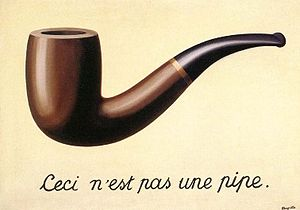
\includegraphics[width=0.4\textwidth,height=0.4\textheight,keepaspectratio]{./Images/MagrittePipe}
\end{frame}

%-----------

\begin{frame}[fragile]\large
\frametitle{Pipes}

Pipe \texttt{\%>\%} is a flow operator. It indicates how the data is passed from one function to another. \bigskip

Consider following analysis:


\begin{knitrout}\footnotesize
\definecolor{shadecolor}{rgb}{0.969, 0.969, 0.969}\color{fgcolor}\begin{kframe}
\begin{alltt}
\hlkwd{rnorm}\hlstd{(}\hlnum{100}\hlstd{)} \hlopt \hlkwd{abs}\hlstd{()} \hlopt \hlkwd{sqrt}\hlstd{()} \hlopt \hlkwd{hist}\hlstd{()}
\end{alltt}
\end{kframe}
\end{knitrout}

\onslide<2-> is equivalent to:
\begin{knitrout}\footnotesize
\definecolor{shadecolor}{rgb}{0.969, 0.969, 0.969}\color{fgcolor}\begin{kframe}
\begin{alltt}
\hlkwd{hist}\hlstd{(}\hlkwd{sqrt}\hlstd{(}\hlkwd{abs}\hlstd{(}\hlkwd{rnorm}\hlstd{(}\hlnum{100}\hlstd{))))}
\end{alltt}
\end{kframe}
\end{knitrout}
\onslide<3->or even to:

\begin{knitrout}\footnotesize
\definecolor{shadecolor}{rgb}{0.969, 0.969, 0.969}\color{fgcolor}\begin{kframe}
\begin{alltt}
\hlstd{normData} \hlkwb{<-} \hlkwd{rnorm}\hlstd{(}\hlnum{100}\hlstd{)}
\hlstd{absData}  \hlkwb{<-} \hlkwd{abs}\hlstd{(normData)}
\hlstd{sqrtData} \hlkwb{<-} \hlkwd{sqrt}\hlstd{(absData)}
\hlkwd{hist}\hlstd{(sqrtData)}
\end{alltt}
\end{kframe}
\end{knitrout}

\end{frame}

%-----------

\begin{frame}[fragile]\large
\frametitle{Function: \texttt{select}}
You want to do an analysis of \textcolor{red}{cyl} and \textcolor{red}{am} from the car dataset. 

\begin{knitrout}\footnotesize
\definecolor{shadecolor}{rgb}{0.969, 0.969, 0.969}\color{fgcolor}\begin{kframe}
\begin{alltt}
\hlstd{dataIn} \hlopt
  \hlkwd{select}\hlstd{(cyl, am)} \hlopt
  \hlkwd{table}\hlstd{()}
\end{alltt}
\begin{verbatim}
##    am
## cyl  0  1
##   4  3  8
##   6  4  3
##   8 12  2
\end{verbatim}
\end{kframe}
\end{knitrout}

\end{frame}

%-----------

\begin{frame}[fragile]\large
\frametitle{Function: \texttt{filter}}
You want to do the same analysis as before, but only with  $hp<150$ \onslide<2->

\begin{knitrout}\footnotesize
\definecolor{shadecolor}{rgb}{0.969, 0.969, 0.969}\color{fgcolor}\begin{kframe}
\begin{alltt}
\hlstd{dataIn} \hlopt
  \hlkwd{filter}\hlstd{(hp} \hlopt{<} \hlnum{150}\hlstd{)} \hlopt
  \hlkwd{select}\hlstd{(cyl, am)} \hlopt
  \hlkwd{table}\hlstd{()}
\end{alltt}
\begin{verbatim}
##    am
## cyl 0 1
##   4 3 8
##   6 4 2
\end{verbatim}
\end{kframe}
\end{knitrout}
\onslide<3-> What is this? $hp == 150$, $hp$ != $150$, $hp >= 150$  
\end{frame}

%-----------

\begin{frame}[fragile]\large
\frametitle{Function: \texttt{filter} - continued}
\begin{itemize}
 \item \texttt{A \& B} means A \textcolor{blue}{AND} B
 \item \texttt{A | B} means A \textcolor{blue}{OR} B
\end{itemize}

You want to do the same analysis as before, but only with $hp<150$ AND $mpg>14$ \onslide<2->

\begin{knitrout}\footnotesize
\definecolor{shadecolor}{rgb}{0.969, 0.969, 0.969}\color{fgcolor}\begin{kframe}
\begin{alltt}
\hlstd{dataIn} \hlopt
  \hlkwd{filter}\hlstd{(hp} \hlopt{<} \hlnum{150} \hlopt{&} \hlstd{mpg} \hlopt{>} \hlnum{14}\hlstd{)} \hlopt
  \hlkwd{select}\hlstd{(cyl, am)} \hlopt
  \hlkwd{table}\hlstd{()}
\end{alltt}
\begin{verbatim}
##    am
## cyl 0 1
##   4 3 8
##   6 4 2
\end{verbatim}
\end{kframe}
\end{knitrout}

\end{frame}

%-----------

\begin{frame}[fragile]\large
\frametitle{Function: \texttt{mutate}.  }
Miles per gallon? We are in Europe! Let's convert it to units which make sense: \smallskip
1 mile $\sim$ 1.61 kilometer, 1 gallon $\sim$ 3.79 liters. 1 mpg $\sim$ 0.42 kmpl

\begin{knitrout}\footnotesize
\definecolor{shadecolor}{rgb}{0.969, 0.969, 0.969}\color{fgcolor}\begin{kframe}
\begin{alltt}
\hlstd{carsData} \hlkwb{<-} \hlstd{dataIn} \hlopt
  \hlkwd{mutate}\hlstd{(}\hlkwc{kmpl} \hlstd{=} \hlnum{0.42}\hlopt{*}\hlstd{mpg)}
\end{alltt}
\end{kframe}
\end{knitrout}
Check whether it worked by displaying \textcolor{blue}{head} of \textcolor{red}{carsData}. Show only name, mpg a and kmpl columns:\onslide<3->
\begin{knitrout}\footnotesize
\definecolor{shadecolor}{rgb}{0.969, 0.969, 0.969}\color{fgcolor}\begin{kframe}
\begin{alltt}
\hlstd{carsData} \hlopt \hlkwd{select}\hlstd{(name, mpg, kmpl)} \hlopt \hlkwd{head}\hlstd{()}
\end{alltt}
\begin{verbatim}
##                name  mpg  kmpl
## 1         Mazda RX4 21.0 8.820
## 2     Mazda RX4 Wag 21.0 8.820
## 3        Datsun 710 22.8 9.576
## 4    Hornet 4 Drive 21.4 8.988
## 5 Hornet Sportabout 18.7 7.854
## 6           Valiant 18.1 7.602
\end{verbatim}
\end{kframe}
\end{knitrout}

\end{frame}

%-----------

\begin{frame}[fragile]\large
\frametitle{Function: \texttt{summarise} }
We want to know: 
\begin{enumerate} 
 \item mean value of kmpl = \textcolor{red}{\texttt{meanKMPL}}
 \item mean value of hp = \textcolor{red}{\texttt{meanHP}}
\end{enumerate}

\begin{knitrout}\footnotesize
\definecolor{shadecolor}{rgb}{0.969, 0.969, 0.969}\color{fgcolor}\begin{kframe}
\begin{alltt}
\hlstd{carsData} \hlopt
  \hlkwd{summarise}\hlstd{(}
    \hlkwc{meanKMPL} \hlstd{=} \hlkwd{mean}\hlstd{(kmpl),}
    \hlkwc{meanHP}   \hlstd{=} \hlkwd{mean}\hlstd{(hp)}
  \hlstd{)}
\end{alltt}
\begin{verbatim}
##   meanKMPL   meanHP
## 1 8.438062 146.6875
\end{verbatim}
\end{kframe}
\end{knitrout}

We have created a new data frame with 2 columns. 
\end{frame}

%-----------

\begin{frame}[fragile]\large
\frametitle{Function: \texttt{group\_by}}
Let's continue with the previous example. You want to do the analysis on subsets/groups by variable: \textcolor{blue}{group\_by}(\textcolor{red}{cyl}) 

\begin{knitrout}\footnotesize
\definecolor{shadecolor}{rgb}{0.969, 0.969, 0.969}\color{fgcolor}\begin{kframe}
\begin{alltt}
\hlstd{carsData} \hlopt
  \hlkwd{group_by}\hlstd{(cyl)} \hlopt
  \hlkwd{summarise}\hlstd{(}
    \hlkwc{meanKMPL} \hlstd{=} \hlkwd{mean}\hlstd{(kmpl),}
    \hlkwc{meanHP}   \hlstd{=} \hlkwd{mean}\hlstd{(hp)}
  \hlstd{)}
\end{alltt}
\begin{verbatim}
## # A tibble: 3 x 3
##     cyl meanKMPL meanHP
##   <int>    <dbl>  <dbl>
## 1     4    11.2    82.6
## 2     6     8.29  122. 
## 3     8     6.34  209.
\end{verbatim}
\end{kframe}
\end{knitrout}

\end{frame}

%-----------

% = = = = = = = = = = = = = = = = = = = = = = = = = = = = = = = = = = = = = = = = = = = = = = = = = =


%-----------

\begin{frame}\Huge\centering
Visualise
\end{frame}

%-----------

\begin{frame}[fragile]
\frametitle{Data Overview}

\begin{knitrout}\footnotesize
\definecolor{shadecolor}{rgb}{0.969, 0.969, 0.969}\color{fgcolor}\begin{kframe}
\begin{alltt}
\hlkwd{str}\hlstd{(dataIn)}
\end{alltt}
\begin{verbatim}
## 'data.frame':	32 obs. of  12 variables:
##  $ name: Factor w/ 32 levels "AMC Javelin",..: 18 19 5 13 14 31 7 21 20 22 ...
##  $ mpg : num  21 21 22.8 21.4 18.7 18.1 14.3 24.4 22.8 19.2 ...
##  $ cyl : int  6 6 4 6 8 6 8 4 4 6 ...
##  $ disp: num  160 160 108 258 360 ...
##  $ hp  : int  110 110 93 110 175 105 245 62 95 123 ...
##  $ drat: num  3.9 3.9 3.85 3.08 3.15 2.76 3.21 3.69 3.92 3.92 ...
##  $ wt  : num  2.62 2.88 2.32 3.21 3.44 ...
##  $ qsec: num  16.5 17 18.6 19.4 17 ...
##  $ vs  : int  0 0 1 1 0 1 0 1 1 1 ...
##  $ am  : int  1 1 1 0 0 0 0 0 0 0 ...
##  $ gear: int  4 4 4 3 3 3 3 4 4 4 ...
##  $ carb: int  4 4 1 1 2 1 4 2 2 4 ...
\end{verbatim}
\end{kframe}
\end{knitrout}

\end{frame}

%-----------

\begin{frame}[fragile]\large
\frametitle{Library \textcolor{blue}{ggplot}}

Library ggplots introduces plotting by layers.

\begin{enumerate}
 \item Define underying layer (data + variables)
 \item Add \textcolor{violet}{\textbf{layers}} (points, boxplots,\ldots)
\end{enumerate}

Every \textcolor{red}{ggplot()} plot contains \textcolor{blue}{data reference} and \textcolor{orange}{\textbf{aes}thetic mapping}.\bigskip

\texttt{\textcolor{red}{ggplot(}\textcolor{blue}{dataIn}, \textcolor{orange}{aes(x=hp, y=mpg)}\textcolor{red}{)}} + \newline
\texttt{\textcolor{violet}{\textbf{\hspace{0.5cm}geom\_point()}}}\smallskip

\end{frame}

%-----------

\begin{frame}[fragile]\centering

\begin{knitrout}\footnotesize
\definecolor{shadecolor}{rgb}{0.969, 0.969, 0.969}\color{fgcolor}\begin{kframe}
\begin{alltt}
\hlkwd{library}\hlstd{(ggplot2)}
\hlkwd{ggplot}\hlstd{(dataIn,} \hlkwd{aes}\hlstd{(}\hlkwc{x}\hlstd{=hp,} \hlkwc{y}\hlstd{=mpg))} \hlopt{+}
  \hlkwd{geom_point}\hlstd{()}
\end{alltt}
\end{kframe}
\includegraphics[width=\maxwidth]{figure/unnamed-chunk-31-1} 

\end{knitrout}

\end{frame}

%-----------

\begin{frame}[fragile]\large
\frametitle{Library ggplot}

What makes ggplot powerful is an application of aestethics:
\begin{itemize}
 \item color
 \item fill
 \item size
 \item shape
 \item linetype
\end{itemize}\bigskip

Take a look at following two plots.

\end{frame}

%-----------

\begin{frame}[fragile]\centering
\frametitle{\texttt{color} as a Graphical Parameter}
\begin{knitrout}\footnotesize
\definecolor{shadecolor}{rgb}{0.969, 0.969, 0.969}\color{fgcolor}\begin{kframe}
\begin{alltt}
\hlkwd{ggplot}\hlstd{(dataIn,} \hlkwd{aes}\hlstd{(}\hlkwc{x}\hlstd{=hp,} \hlkwc{y}\hlstd{=mpg))} \hlopt{+}
  \hlkwd{geom_point}\hlstd{(}\hlkwc{color}\hlstd{=}\hlstr{"blue"}\hlstd{)}
\end{alltt}
\end{kframe}
\includegraphics[width=\maxwidth]{figure/unnamed-chunk-32-1} 

\end{knitrout}

\end{frame}

%-----------

\begin{frame}[fragile]\centering
\frametitle{\texttt{color} as an \texttt{aes}tetics}

\begin{knitrout}\footnotesize
\definecolor{shadecolor}{rgb}{0.969, 0.969, 0.969}\color{fgcolor}\begin{kframe}
\begin{alltt}
\hlkwd{ggplot}\hlstd{(dataIn,} \hlkwd{aes}\hlstd{(}\hlkwc{x}\hlstd{=hp,} \hlkwc{y}\hlstd{=mpg,} \hlkwc{color}\hlstd{=cyl))} \hlopt{+}
  \hlkwd{geom_point}\hlstd{()}
\end{alltt}
\end{kframe}
\includegraphics[width=\maxwidth]{figure/unnamed-chunk-33-1} 

\end{knitrout}

\end{frame}

%-----------

\begin{frame}[fragile]\centering

\begin{knitrout}\footnotesize
\definecolor{shadecolor}{rgb}{0.969, 0.969, 0.969}\color{fgcolor}\begin{kframe}
\begin{alltt}
\hlstd{dataIn} \hlopt
  \hlkwd{mutate}\hlstd{(}\hlkwc{cyl} \hlstd{=} \hlkwd{factor}\hlstd{(cyl))} \hlopt
 \hlkwd{ggplot}\hlstd{(.,} \hlkwd{aes}\hlstd{(}\hlkwc{x}\hlstd{=hp,} \hlkwc{y}\hlstd{=mpg,} \hlkwc{color}\hlstd{=cyl))} \hlopt{+}
  \hlkwd{geom_point}\hlstd{()}
\end{alltt}
\end{kframe}
\includegraphics[width=\maxwidth]{figure/unnamed-chunk-34-1} 

\end{knitrout}

\end{frame}

%-----------

\begin{frame}[fragile]\large

We can adjust (almost) everything in ggplot through additional functions (just to mention few):

\begin{itemize}
 \item \texttt{facet\_grid()}
 \item \texttt{scale\_y\_continuous(name, limits, ...)}, \texttt{scale\_x\_discrete()}
 \item \texttt{theme\_bw()}
\end{itemize}

\end{frame}

%-----------

\begin{frame}[fragile]\centering

\begin{knitrout}\footnotesize
\definecolor{shadecolor}{rgb}{0.969, 0.969, 0.969}\color{fgcolor}\begin{kframe}
\begin{alltt}
\hlstd{dataIn} \hlopt
  \hlkwd{mutate}\hlstd{(}\hlkwc{cyl} \hlstd{=} \hlkwd{as.factor}\hlstd{(cyl))} \hlopt
 \hlkwd{ggplot}\hlstd{(.,} \hlkwd{aes}\hlstd{(}\hlkwc{x}\hlstd{=hp,} \hlkwc{y}\hlstd{=mpg))} \hlopt{+}
  \hlkwd{geom_point}\hlstd{()} \hlopt{+}
  \hlkwd{scale_x_continuous}\hlstd{(}\hlstr{"Power of cars in car dataset. [hp]"}\hlstd{)} \hlopt{+}
  \hlkwd{facet_grid}\hlstd{(.}\hlopt{~}\hlstd{cyl)} \hlopt{+}
  \hlkwd{theme_bw}\hlstd{()}
\end{alltt}
\end{kframe}
\includegraphics[width=\maxwidth]{figure/unnamed-chunk-35-1} 

\end{knitrout}

\end{frame}

%-----------

\begin{frame}[fragile]\centering
\frametitle{Why not to add regressions by \texttt{geom\_smooth()}?}
\begin{knitrout}\footnotesize
\definecolor{shadecolor}{rgb}{0.969, 0.969, 0.969}\color{fgcolor}\begin{kframe}
\begin{alltt}
\hlstd{dataIn} \hlopt
  \hlkwd{mutate}\hlstd{(}\hlkwc{cyl} \hlstd{=} \hlkwd{as.factor}\hlstd{(cyl))} \hlopt
 \hlkwd{ggplot}\hlstd{(.,} \hlkwd{aes}\hlstd{(}\hlkwc{x}\hlstd{=hp,} \hlkwc{y}\hlstd{=mpg))} \hlopt{+} \hlkwd{geom_point}\hlstd{()} \hlopt{+}
  \hlkwd{scale_x_continuous}\hlstd{(}\hlstr{"Power of cars in car dataset. [hp]"}\hlstd{)} \hlopt{+}
  \hlkwd{facet_grid}\hlstd{(.}\hlopt{~}\hlstd{cyl)} \hlopt{+} \hlkwd{theme_bw}\hlstd{()} \hlopt{+} \hlkwd{geom_smooth}\hlstd{(}\hlkwc{method}\hlstd{=}\hlstr{"lm"}\hlstd{)}
\end{alltt}
\end{kframe}
\includegraphics[width=\maxwidth]{figure/unnamed-chunk-36-1} 

\end{knitrout}

\end{frame}

%-----------

\begin{frame}[fragile]\centering
\frametitle{\texttt{geom\_boxplot}}
\begin{knitrout}\footnotesize
\definecolor{shadecolor}{rgb}{0.969, 0.969, 0.969}\color{fgcolor}\begin{kframe}
\begin{alltt}
\hlstd{dataIn} \hlopt
  \hlkwd{mutate}\hlstd{(}\hlkwc{cyl} \hlstd{=} \hlkwd{as.factor}\hlstd{(cyl))} \hlopt
 \hlkwd{ggplot}\hlstd{(}\hlkwd{aes}\hlstd{(}\hlkwc{x}\hlstd{=cyl,} \hlkwc{y}\hlstd{=mpg) )} \hlopt{+}
  \hlkwd{geom_boxplot}\hlstd{()}
\end{alltt}
\end{kframe}
\includegraphics[width=\maxwidth]{figure/unnamed-chunk-37-1} 

\end{knitrout}

\end{frame}

%-----------

\begin{frame}[fragile]\centering
\frametitle{Let's add additional layer}
\begin{knitrout}\footnotesize
\definecolor{shadecolor}{rgb}{0.969, 0.969, 0.969}\color{fgcolor}\begin{kframe}
\begin{alltt}
\hlstd{dataIn} \hlopt
  \hlkwd{mutate}\hlstd{(}\hlkwc{cyl} \hlstd{=} \hlkwd{as.factor}\hlstd{(cyl))} \hlopt
 \hlkwd{ggplot}\hlstd{(}\hlkwd{aes}\hlstd{(}\hlkwc{x}\hlstd{=cyl,} \hlkwc{y}\hlstd{=mpg) )} \hlopt{+}
  \hlkwd{geom_boxplot}\hlstd{()} \hlopt{+}
  \hlkwd{geom_point}\hlstd{()}
\end{alltt}
\end{kframe}
\includegraphics[width=\maxwidth]{figure/unnamed-chunk-38-1} 

\end{knitrout}

\end{frame}

%-----------

\begin{frame}[fragile]\centering
\frametitle{Add geom-specific aes}
\begin{knitrout}\footnotesize
\definecolor{shadecolor}{rgb}{0.969, 0.969, 0.969}\color{fgcolor}\begin{kframe}
\begin{alltt}
\hlstd{dataIn} \hlopt
  \hlkwd{mutate}\hlstd{(}\hlkwc{cyl} \hlstd{=} \hlkwd{as.factor}\hlstd{(cyl))} \hlopt
 \hlkwd{ggplot}\hlstd{(}\hlkwd{aes}\hlstd{(}\hlkwc{x}\hlstd{=cyl,} \hlkwc{y}\hlstd{=mpg) )} \hlopt{+}
  \hlkwd{geom_boxplot}\hlstd{()} \hlopt{+}
  \hlkwd{geom_jitter}\hlstd{(}\hlkwc{alpha}\hlstd{=}\hlnum{0.25}\hlstd{)}
\end{alltt}
\end{kframe}
\includegraphics[width=\maxwidth]{figure/unnamed-chunk-39-1} 

\end{knitrout}

\end{frame}

%-----------

\begin{frame}[fragile]\centering
\frametitle{Add geom-specific aes}
\begin{knitrout}\footnotesize
\definecolor{shadecolor}{rgb}{0.969, 0.969, 0.969}\color{fgcolor}\begin{kframe}
\begin{alltt}
\hlstd{dataIn} \hlopt
  \hlkwd{mutate}\hlstd{(}\hlkwc{cyl} \hlstd{=} \hlkwd{as.factor}\hlstd{(cyl))} \hlopt
 \hlkwd{ggplot}\hlstd{(}\hlkwd{aes}\hlstd{(}\hlkwc{x}\hlstd{=cyl,} \hlkwc{y}\hlstd{=mpg) )} \hlopt{+}
  \hlkwd{geom_boxplot}\hlstd{()} \hlopt{+}
  \hlkwd{geom_jitter}\hlstd{(}\hlkwd{aes}\hlstd{(}\hlkwc{size}\hlstd{=hp),} \hlkwc{alpha}\hlstd{=}\hlnum{0.25}\hlstd{)}
\end{alltt}
\end{kframe}
\includegraphics[width=\maxwidth]{figure/unnamed-chunk-40-1} 

\end{knitrout}

\end{frame}

%-----------

\begin{frame}[fragile]
\frametitle{Processing ggplots}
\begin{knitrout}
\definecolor{shadecolor}{rgb}{0.969, 0.969, 0.969}\color{fgcolor}\begin{kframe}
\begin{alltt}
\hlstd{plot1} \hlkwb{<-} \hlstd{dataIn} \hlopt
  \hlkwd{mutate}\hlstd{(}\hlkwc{cyl} \hlstd{=} \hlkwd{as.factor}\hlstd{(cyl))} \hlopt
 \hlkwd{ggplot}\hlstd{(}\hlkwd{aes}\hlstd{(}\hlkwc{x}\hlstd{=cyl,} \hlkwc{y}\hlstd{=mpg) )} \hlopt{+}
  \hlkwd{geom_boxplot}\hlstd{()} \hlopt{+}
  \hlkwd{geom_point}\hlstd{()}

\hlstd{plot1}
\hlkwd{ggsave}\hlstd{(}\hlstr{"./images/myPlot1.pdf"}\hlstd{,} \hlkwc{width}\hlstd{=}\hlnum{6}\hlstd{,} \hlkwc{height} \hlstd{=} \hlnum{4}\hlstd{)} \hlcom{# png, jpeg, ... }
\end{alltt}
\end{kframe}
\end{knitrout}

Try following:

\begin{knitrout}
\definecolor{shadecolor}{rgb}{0.969, 0.969, 0.969}\color{fgcolor}\begin{kframe}
\begin{alltt}
\hlkwd{library}\hlstd{(plotly)}
\hlkwd{ggplotly}\hlstd{(plot1)}
\end{alltt}
\end{kframe}
\end{knitrout}

\end{frame}


%-----------

\begin{frame}\large
\frametitle{Your Turn}

There is a dataset in ggplot library called \texttt{diamonds}.  

\begin{enumerate}
 \item familiarise yourselves with the dataset: \texttt{?diamonds}
 \item how many observations is in the dataset? Find this information in R!
 \item Create a table from the main dataset which analyses price of diamonds and visualise it in ggplot.
 \item Try to combine filter, group\_by and \textbf{summarise}
\end{enumerate}
\end{frame}

%-----------

% = = = = = = = = = = = = = = = = = = = = = = = = = = = = = = = = = = = = = = = = = = = = = = = = = =


%-----------

\begin{frame}
\begin{columns}[T] % align columns
\begin{column}{.48\textwidth}
%\rule{\linewidth}{4pt}
\vspace{2cm}
 \begin{itemize}
  \item Book about R
  \item and good DS practices.
  \item Online version available \textcolor{orange}{\href{http://r4ds.had.co.nz/}{here}}.
 \end{itemize}
\end{column}%
\hfill%
\begin{column}{.48\textwidth}
%\color{blue}\rule{\linewidth}{4pt}

 
\includegraphics[width=\textwidth,height=\textheight,keepaspectratio]{./Images/02_rBook}
\end{column}%
\end{columns}
\end{frame}

%-----------

\begin{frame}\centering\Large
Thank you! \bigskip 

homolka@utb.cz\bigskip 

\href{https://github.com/luboRprojects/tidyWorkshop}{
\includegraphics[width=0.1\textwidth,height=0.1\textheight,keepaspectratio]{./Images/github}}


%\href{https://stackoverflow.com/users/7357438/lstat?tab=profile}{\includegraphics[width=0.3\textwidth,height=0.3\textheight,keepaspectratio]{./Images/stackoverflow}}

\end{frame}

\end{document}
